\chapter{Analysis}

\section{Introduction}

Client: Neil Green
Job Description: Owns and manages an Independently run gym
Contact Information: Sweat Gymnasium LLP
					 107a Clay Street
					 Soham
					 Ely
					 Cambridgeshire
					 CB7 5HL

					 Telephone: 01353 721864
					 Email: info@sweatgym.co.uk

\subsection{Client Identification}

My client is an independent gym owner who is struggling to keep track of his members payment details and use of the facilities. He is also my brother in law. He approached me about creating a system for him after I mentioned I needed a client for coursework and he mentioned that he is having issues with clients not paying him since he doesn't have an accurate, reliable system for keeping track of payments.

\subsection{Define the current system}

His current system involves using a series of excel spreadsheets to document his clients payment, membership details, personal details and exercise plans. He does this manually by creating new spreadsheets and entering the clients data by hand. His clients give him this data by filling out a membership form and membership agreement and via discussion and interview if they need an exercise program made for them. My client uses one spreadsheet to keep a record of all the members of the gym including details like their member ID, their contact information, payment information and their membership details as well as whether their up to date with payments. Each member then has their own spreadsheet which is used to keep track of any exercise routines they may have paid to have planned for them.

\subsection{Describe the problems}

This system imposes some limitations. First of all, all the processes have to be dealt with manually through spreadsheets without anything other than lack of human error to point out a mistake or notify if someone isn't up to date with payment. This also isn't secure as any piece of information can be changed at any time and to be sure of everything debit mandates would have to be looked over, but even then some clients may have payed by cash and thus wouldn't be recoverable. Their is also the possibility of a computer error that could delete all the documents as they are not backed up anywhere. His gym also know accommodates over 1000 members meaning that he has a large number of spreadsheets for all his clients as well as having his main spreadsheet being exceptionally large meaning the program can lag, especially since the program isn't running on the greatest available hardware. Another issue is that it can be difficult to sort through and search the spreadsheets to find specific information regarding clients, for example if he needs to find they're contact information, excel doesn't have a tool to easily search for that.

\subsection{Section appendix}

Q. What is your current system?

Our current system involves entering data regarding our clients into excel spreadsheets to keep track of the data we need

Q. And what data is it that you record?

We use the first spreadsheet to record our clients names, contact information, payment details, and what membership they have. Each member then has their own spreadsheet for us to detail any exercise plans that they request for us to create. 

Q. What are the limitations of this?
This system means that everything has to be done manually and I won't know if Iv'e forgotten to enter whether someones paid or not as their is no way for me to know if I forgot to change part of the spreadsheet or if my client is trying not to pay. It also isn't very secure as anyone could edit it easily. The process can also be very time consuming.

Q. Is their any additional data you would like to be recorded in the new system?
I would like to be able to store all of the clients information in one place instead of having to use multiple spreadsheets so I can organise all my data more easily. Though i'm pretty sure I don't need any additional information.

Q. What processes do you normally go through with your current system and how do you implement it?
To use my current system I ask my clients to fill out two forms (presented in the investigation section) and then take the information they filled out and enter them digitally into the appropriate excel spreadsheets.

Q.How would you like to operate the new system?
I would like to be able to operate the system similar to how I operate my current one with me being able to enter information from forms my clients filled out, or perhaps even with digital forms I can email them to fill out.

Q.What Inputs and outputs would your new system need? 
I would like to be able to print out a clients information easily in an organised fashion and also be able to create print outs of any other information I would like, possibly to create an invoice or general report for the client. I would also need some physical forms if possible for my less technically inclined members.

Q. What hardware would this need to run on?
This would be run off a reasonably mid spec laptop purchased four years ago. All I really know is it has an i5 processor.

\section{Investigation}


\subsection{The current system}

The current system is made of completely manual functions only using computers for data entry and storing the spreadsheets in which the data is entered. I do my best to explain this system below through the use of hierarchy charts, flowcharts, data flow diagrams and the all the physical and digital forms used in the process.

\subsubsection{Data sources and destinations}

\begin{figure}[H]
    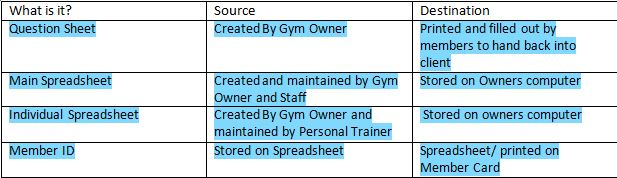
\includegraphics[width=\textwidth]{InvestigationTable1.jpg}
    \caption{Data Sources and Destinations for the current system} \label{fig:Current Destinations}
\end{figure}

\subsubsection{Algorithms}

Hierarchy Charts

Gym Sign Up Process
\begin{python}
1. Information is attained from the client
	1.1 My client gives a form to their client to be promptly filled out
	1.2 The client then hands the sheet back into reception 
	1.3 The information provided on this sheets then enter manually into an excel spreadsheet
	1.4 Do they have an exercise plan? Then the plan is created based on an interview with the client
2.Create Membership Card
	2.1 Make sure all necessary details are correct
	2.2 print Membership card 
\end{python}

Payment Process
\begin{python}
1. Client enters
2. Are they paying upfront?
2.1. Process their payment
2.2. Enter the appropriate information into the correct spreadsheet
2.3 Allow them into the facility
3. Have they payed by direct debit?
3.1. Check to see if the payment went through
3.2. If it did allow them into the facility
3.3 If the payment didnt go through then ask them to pay upfront and return to section 2
3.4 If they refuse to pay ask them to leave
\end{python}

Pseudocode

\begin{python}
Gym Sign Up Process

START

Function GetInfo:
	Client fills out form
	Hands form into gym owner
	Owner enters the information into an excel spreadsheet
	IF they have an exercise plan:
		Owner creates a plan based on an interview with client and enters this into it’s
own spreadsheet
	Owner creates Membership Card
	Owner checks to make sure all the info is correct
	Owner prints membership card and gives it to the new member

GetInfo

END


Payment Process

Start

Function ClientPayment:
	Client enters
	IF paying upfront:
		PayingUpFront
	IF paying by direct debit:
		PayingDirectDebit
	IF they refuse to pay:
		AskThemToLeave

Function PayingUpFront:
	Owner processes payment
	Process their payment
	Enter payment information into the appropriate spreadsheet
	Allow them into the facility

Function PayingDirectDebit:
	Check to see if the payment went through
	IF payment didn’t go through:
		IF they want to pay up front:
			PayingUpFront
		ELSE IF they refuse to pay:
			AskThemToLeave
	ELSE IF the payment did go through:
		Allow them into the facility

Function AskThemToLeave:
	Ask them to leave

ClientPayment 

END
\end{python}

Flow Charts

\begin{figure}[H]
    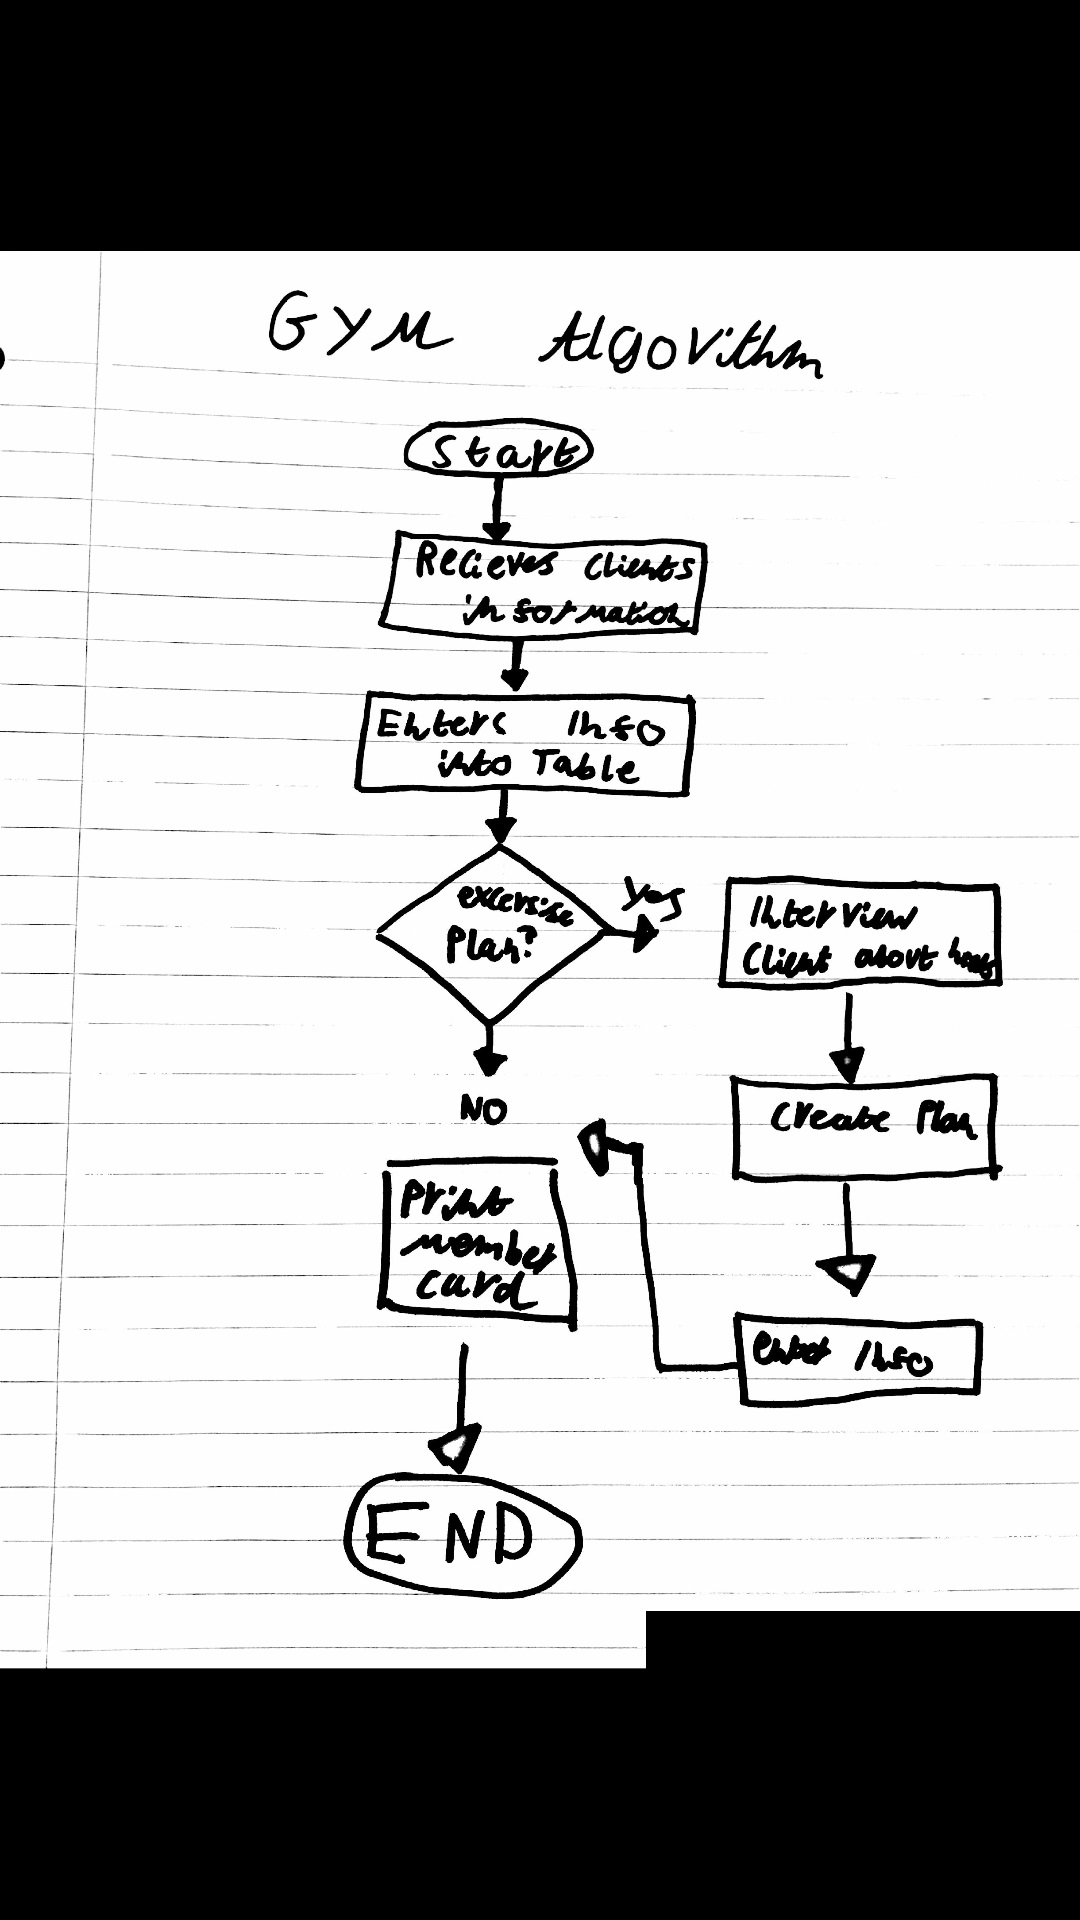
\includegraphics[width=\textwidth]{GymAlgorithm.jpg}
    \caption{Algorithm for the gym sign up process} \label{fig:Algorithm for the gym sign up process}
\end{figure}

\begin{figure}[H]
    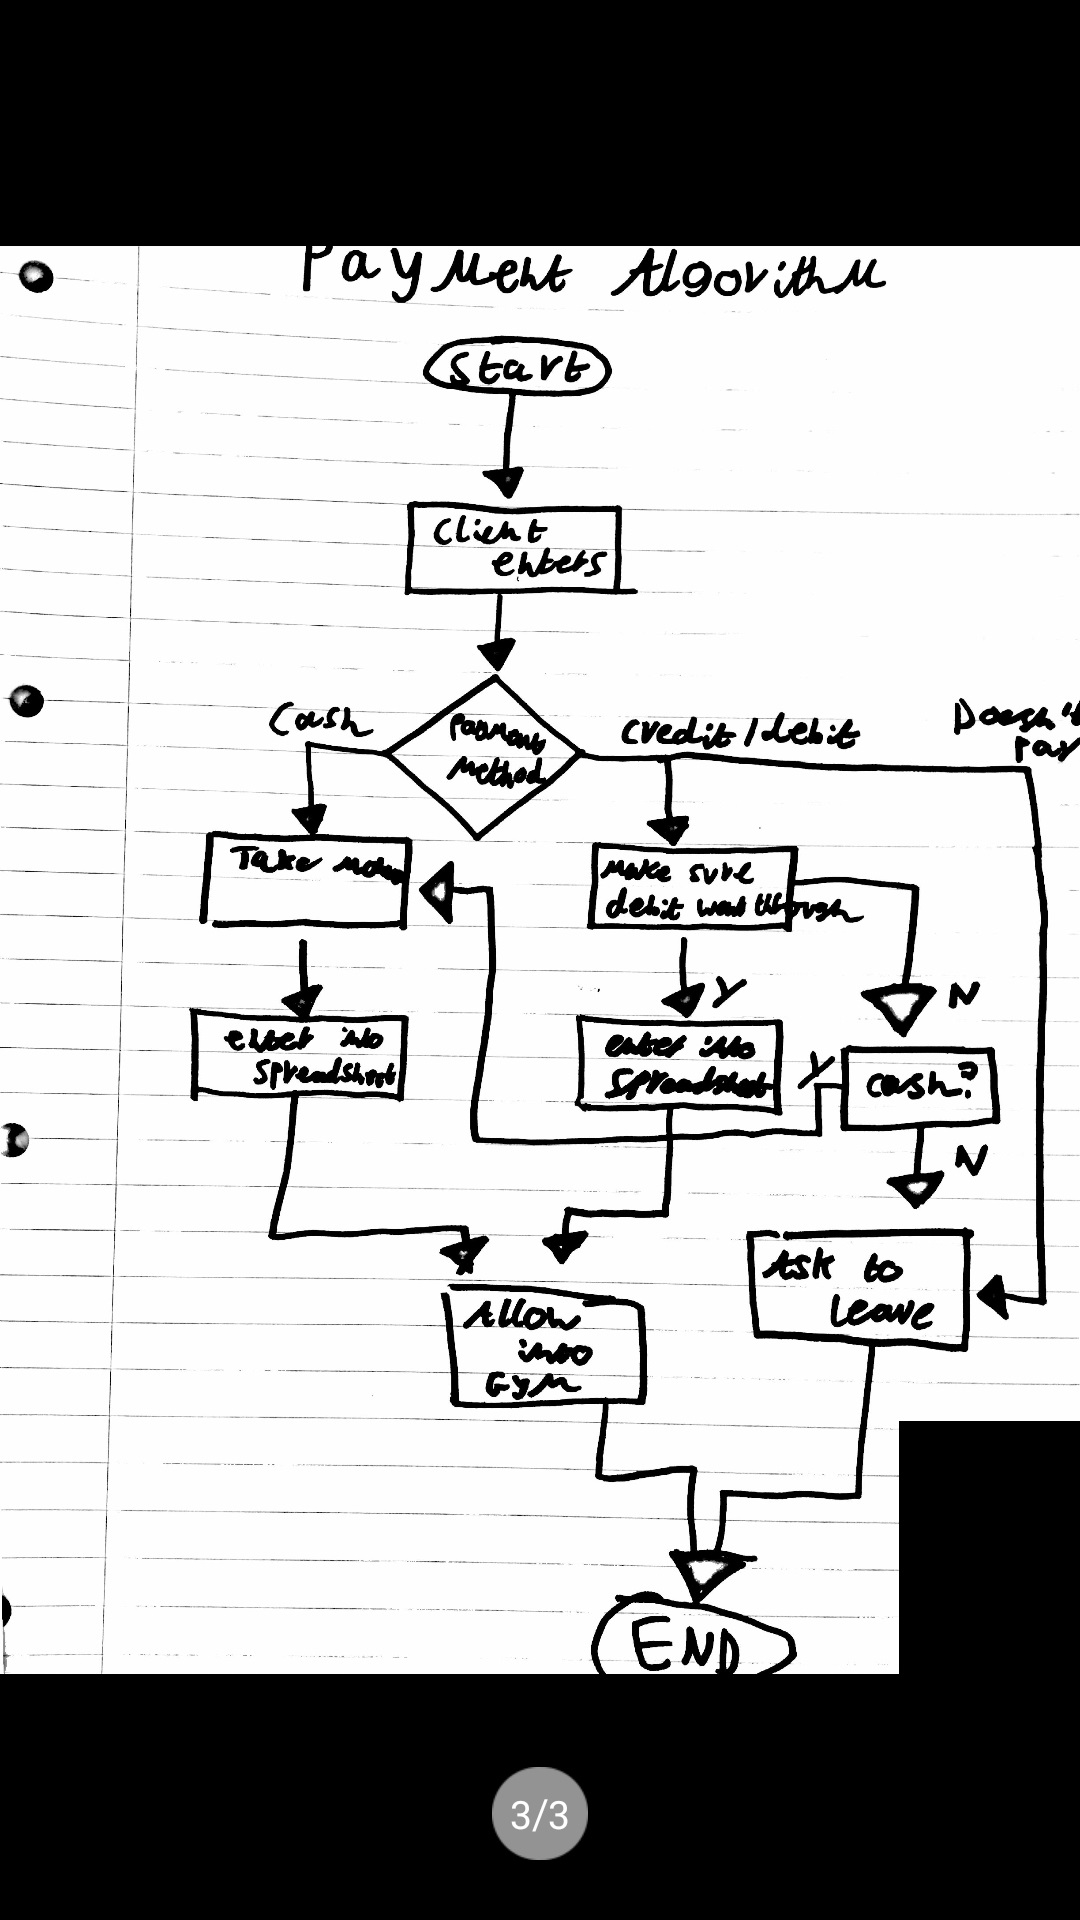
\includegraphics[width=\textwidth]{PaymentAlgorithm.jpg}
    \caption{Algorithm for the payment process} \label{fig:Algorithm for the payment process}
\end{figure}

\subsubsection{Data flow diagram}

\begin{figure}[H]
    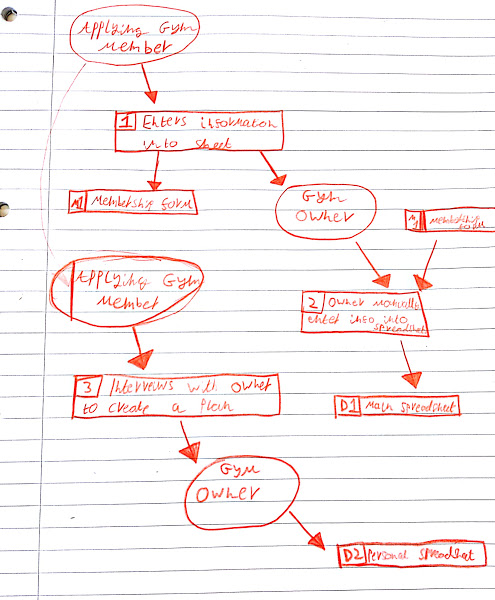
\includegraphics[width=\textwidth]{ProposedDFD.jpg}
    \caption{Data Flow Diagram For The Proposed System} \label{fig:Data Flow Diagram For The Proposed System}
\end{figure}


\subsubsection{Input Forms, Output Forms, Report Formats}

\begin{figure}[H]
    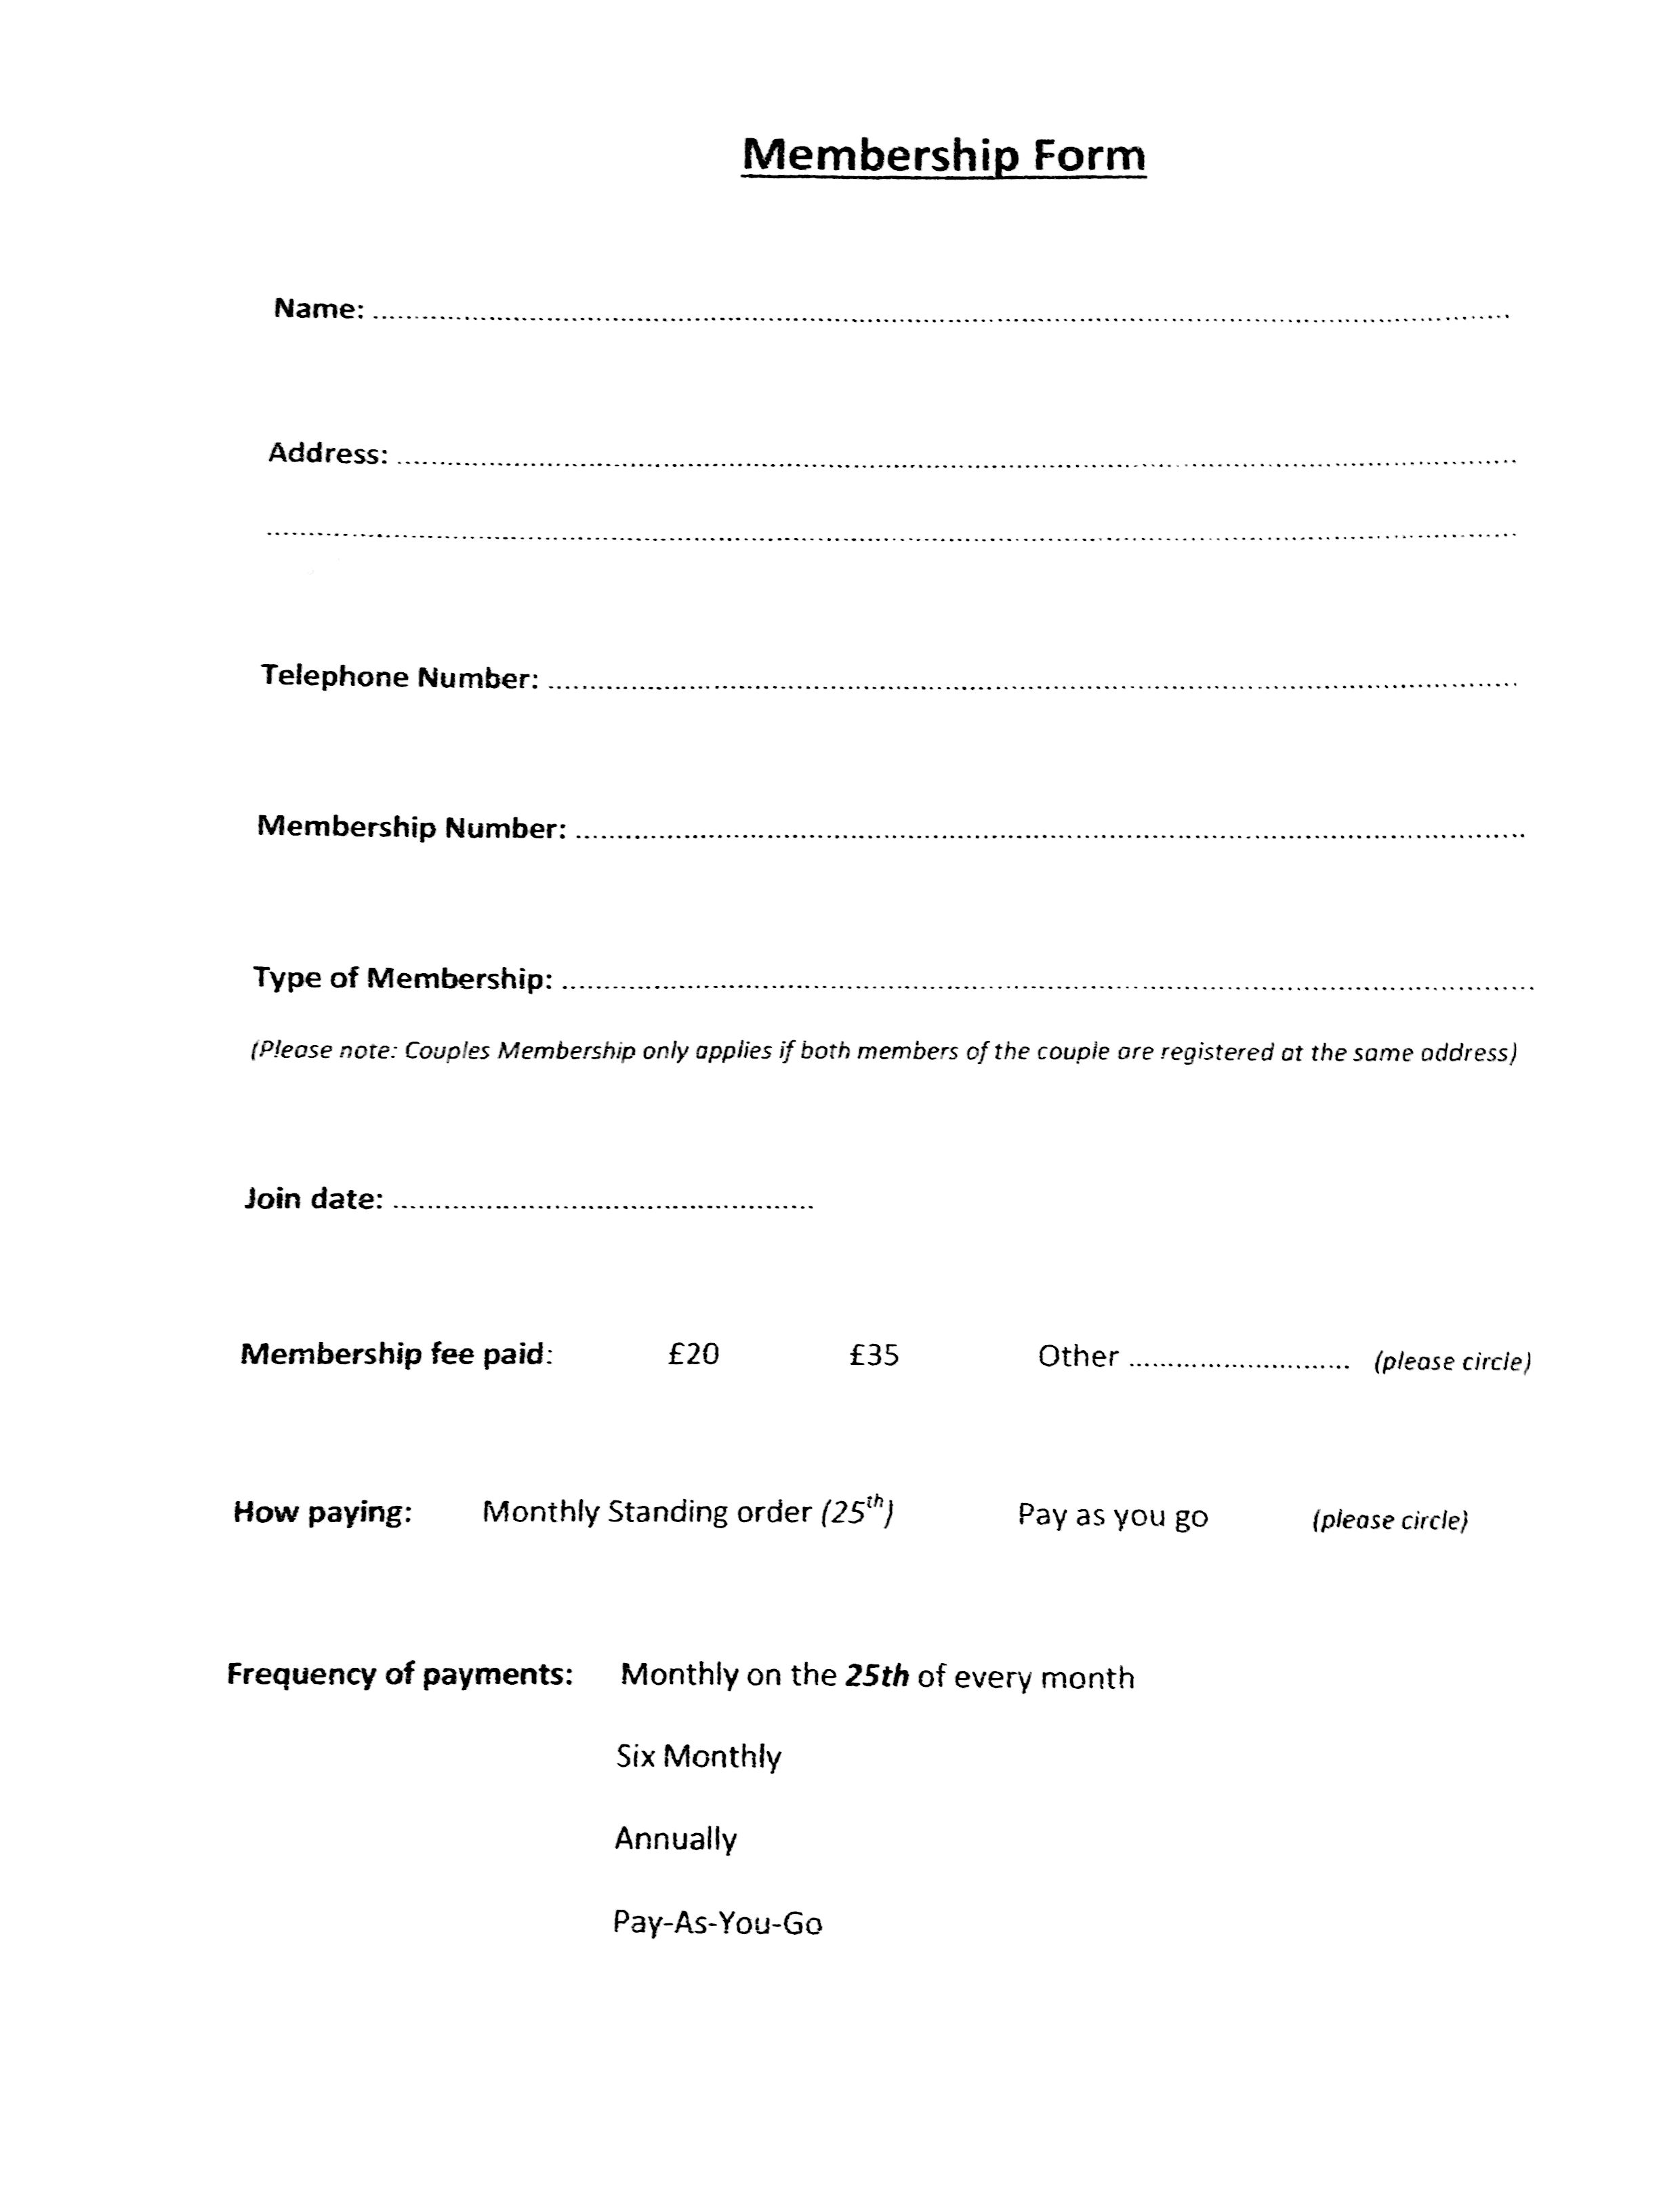
\includegraphics[width=\textwidth]{MembershipForm.jpg}
    \caption{Membership Sign up form} \label{fig:Membership Sign up Form}
\end{figure}

\begin{figure}[H]
    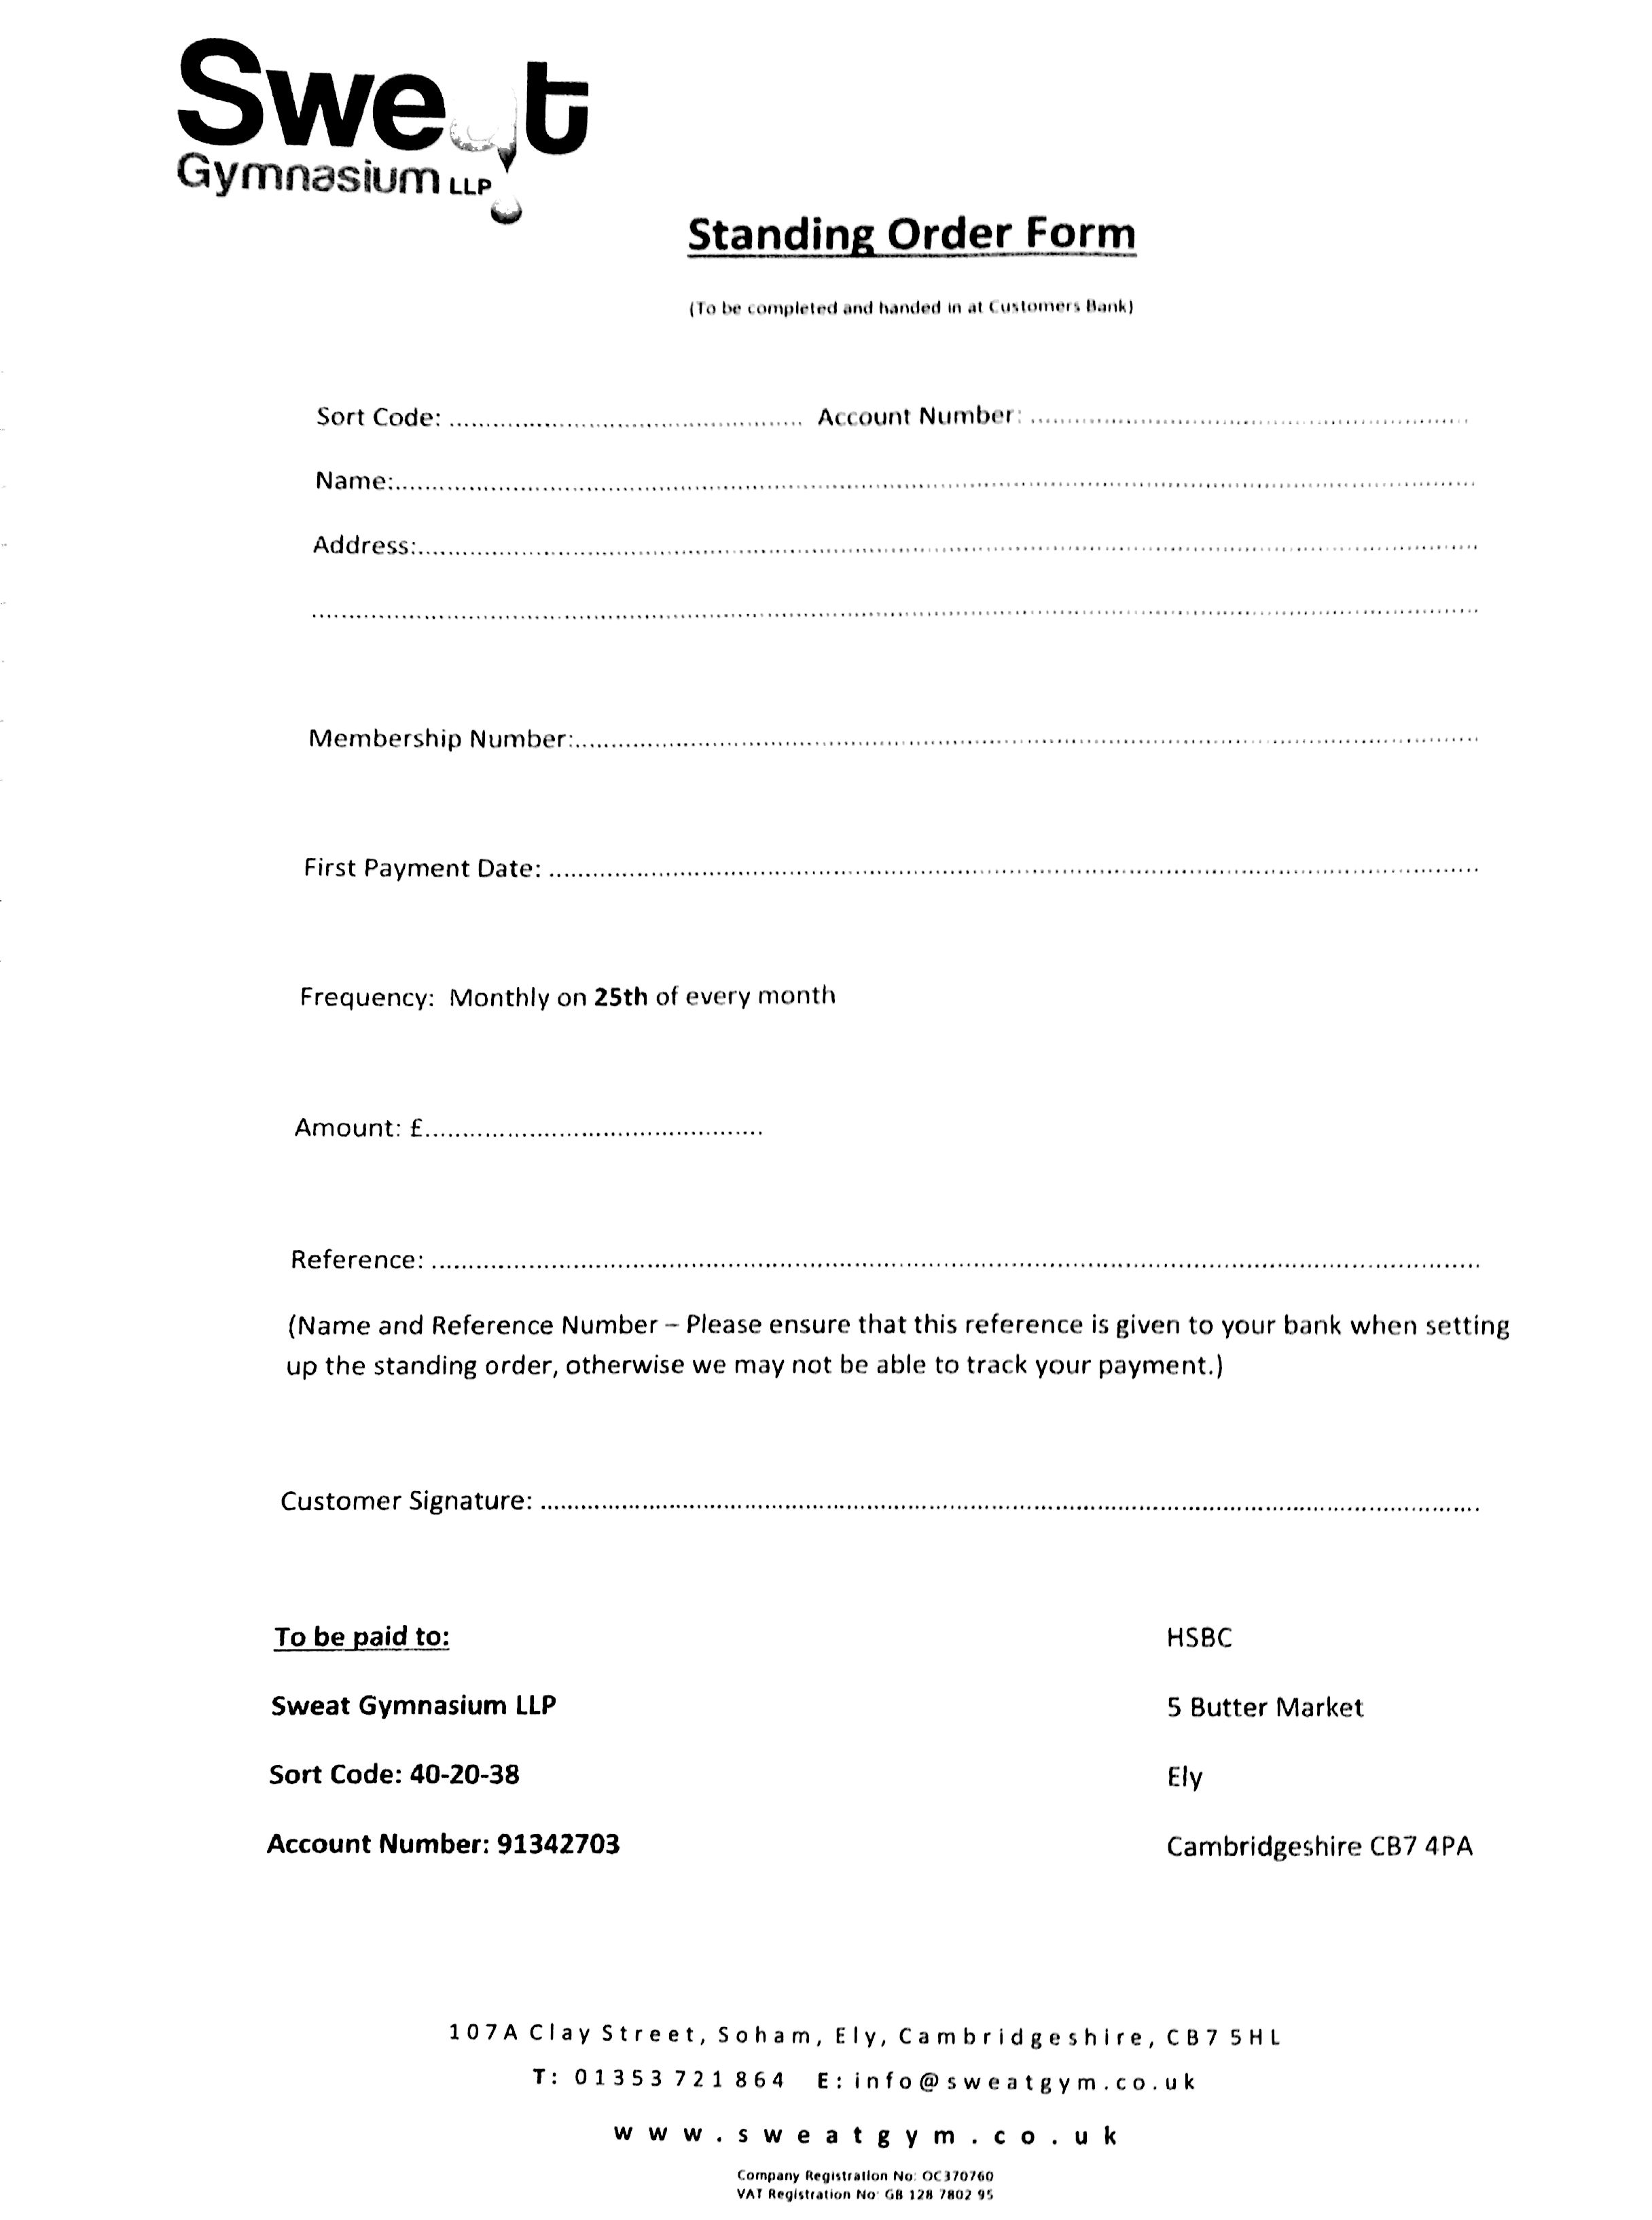
\includegraphics[width=\textwidth]{StandingOrderForm,jpeg.jpg}
    \caption{Standing Order Form} \label{fig:Standing Order Form }
\end{figure}

\subsection{The proposed system}

My proposed system uses a database to keep track of all the data that my client previously kept in an excel spreadsheet using a program created in the python programming language using the PyQt 4 library. This is because its the language I'm most comfortable with and allows for the creation of intuitive UI and the creation of an executable program using the software cx freeze ensuring that the system will be easily usable by my client.

\subsubsection{Data sources and destinations}

\begin{figure}[H]
    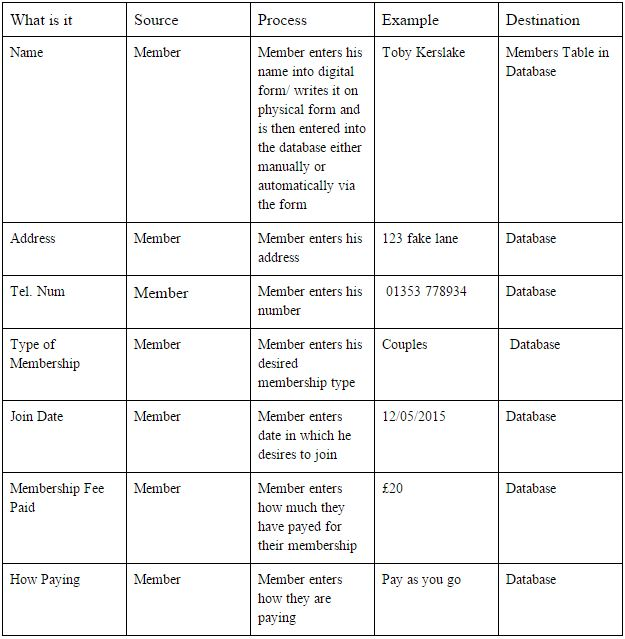
\includegraphics[width=\textwidth]{ProposedSources.jpg}
    \caption{Data Sources and Destinations} \label{fig: Data Sources and Destinations }
\end{figure}

\begin{figure}[H]
    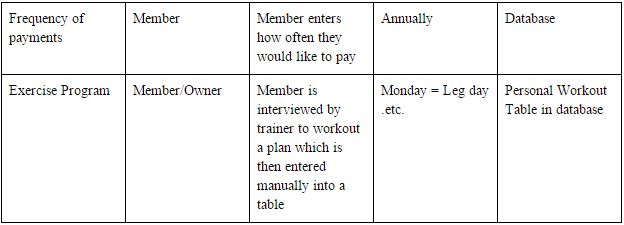
\includegraphics[width=\textwidth]{ProposedSources2.jpg}
    \caption{Data Sources and Destinations 2} \label{fig: Data Sources and Destinations 2 }
\end{figure}

\subsubsection{Data flow diagram}

\begin{figure}[H]
    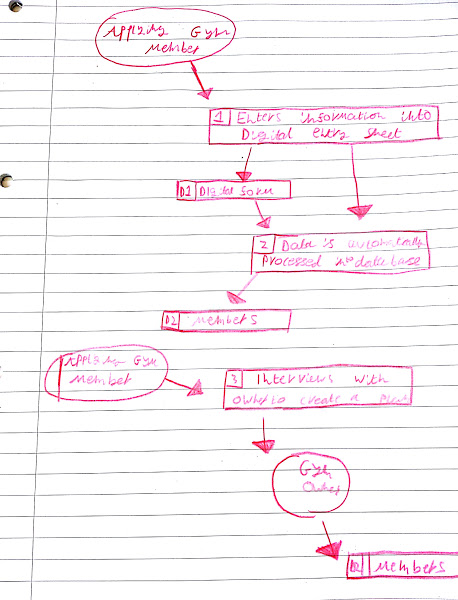
\includegraphics[width=\textwidth]{ProposedDFD2.jpg}
    \caption{Data Flow Diagram} \label{fig: Data Flow Diagram }
\end{figure}

\subsubsection{Data dictionary}

\begin{figure}[H]
    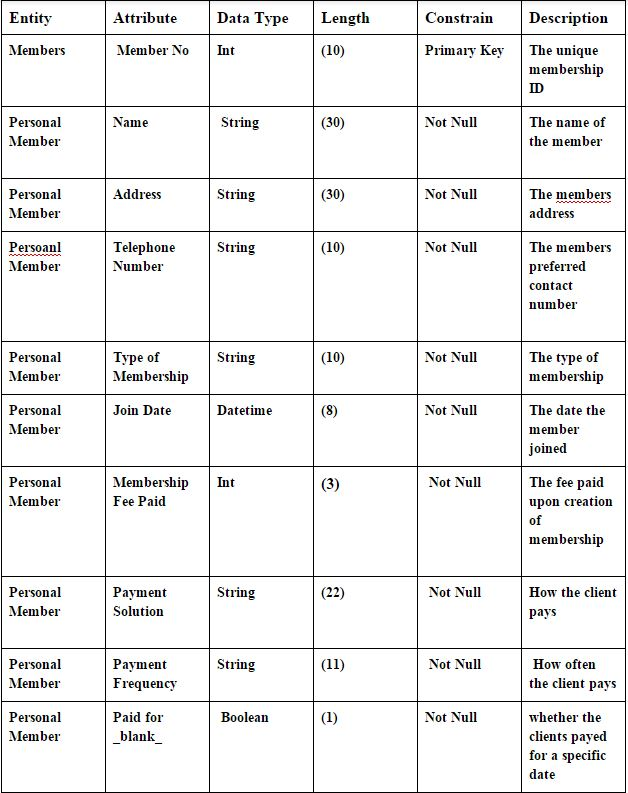
\includegraphics[width=\textwidth]{Sources.jpg}
    \caption{Data Destinations and Sources} \label{fig: Data Destinations and Sources }
\end{figure}

\begin{figure}[H]
    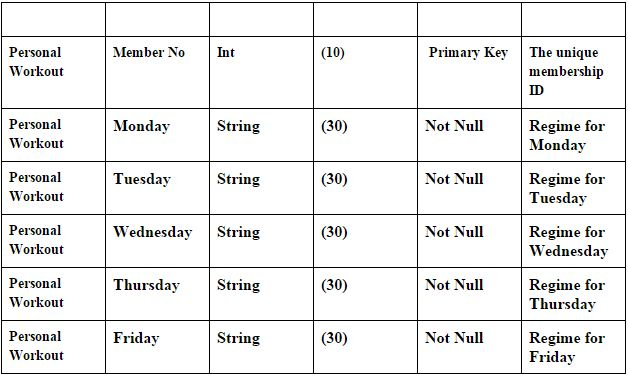
\includegraphics[width=\textwidth]{Sources2.jpg}
    \caption{Data Destinations and Sources 2} \label{fig: Data Destinations and Sources 2 }
\end{figure}

\subsubsection{Volumetrics}

I have decided on an initial size of 2000 members since the gym is nearing that number of members and will inevitably achieve this amount of clients.  My client has said the amount of clients he gains isn't consistent as people often register in different sized groups. The size of the database can be increased at a later date when needed.  

Each member has 11 - 16 fields of data in total, with each data field taking up 1 KB of data.

16 * 1KB * 2000 = 32000 KB
32000 / 1024 = 31.25 MB

The rest of the system should take up a small amount of space that will probably take up about 3MB.

31.25 MB + 3MB = 34.25 MB

\section{Objectives}

\subsection{General Objectives}

    \begin{itemize}  

        \item Clear/easy to understand layout structure for member/client records viewing/observation 

        \item Clear/easy to understand layout structure for all member/client data input  

        \item Clear/easy to understand layout for creating and printing invoices/ member records
        
        \item Clear/easy to understand digital/physical input forms for users to enter data

    \end{itemize}

\subsection{Specific Objectives}

Client/Member Record Viewing/Data Input

\begin{itemize}  

        \item Easy to use Simple Gui with clearly labelled buttons to choose an option (as shown in the mock-ups I presented my client).
        \item Their should be buttons for opening a table, add to it, editing it, deleting an item, creating an invoice or physical record, and searching for something specific.
        \item Each of these buttons should open up either drop down menus or entirely new windows, depending on which is more user friendly, and display further options within those commands.
        \item The interface for entering new information should be easy to use and clearly labelled for adding each attribute to the specified table.
        \item Their should be an easy/ifficient way to switch and search between all of the tables in the database.
    \end{itemize}


System Outputs

\begin{itemize}  

        \item Easy to create reports containing all of a specific clients information in an organised manner on as little paper as legibly possible.
        \item Easy to create invoices for members based off of the information stored in the tables.
\end{itemize}

Input Forms

    \begin{itemize}  

        \item Easy to fill out digital input forms, maybe made in HTML that can be distributed by email or through the gyms website that the program could automatically search for a recieve when being opened.
        \item Printable versions off these forms that can be created to be filled out by hand by less technically inclined clients that can then have their information manually entered into the system by a member of staff.

    \end{itemize}

\subsection{Core Objectives}

\begin{itemize}
    \item Client/Member Record Viewing/Data Input
    \item System Outputs
\end{itemize}


\subsection{Other Objectives}

\begin{itemize}
    \item Input Forms
\end{itemize}

\section{ER Diagrams and Descriptions}


\subsection{ER Diagram}

\begin{figure}[H]
    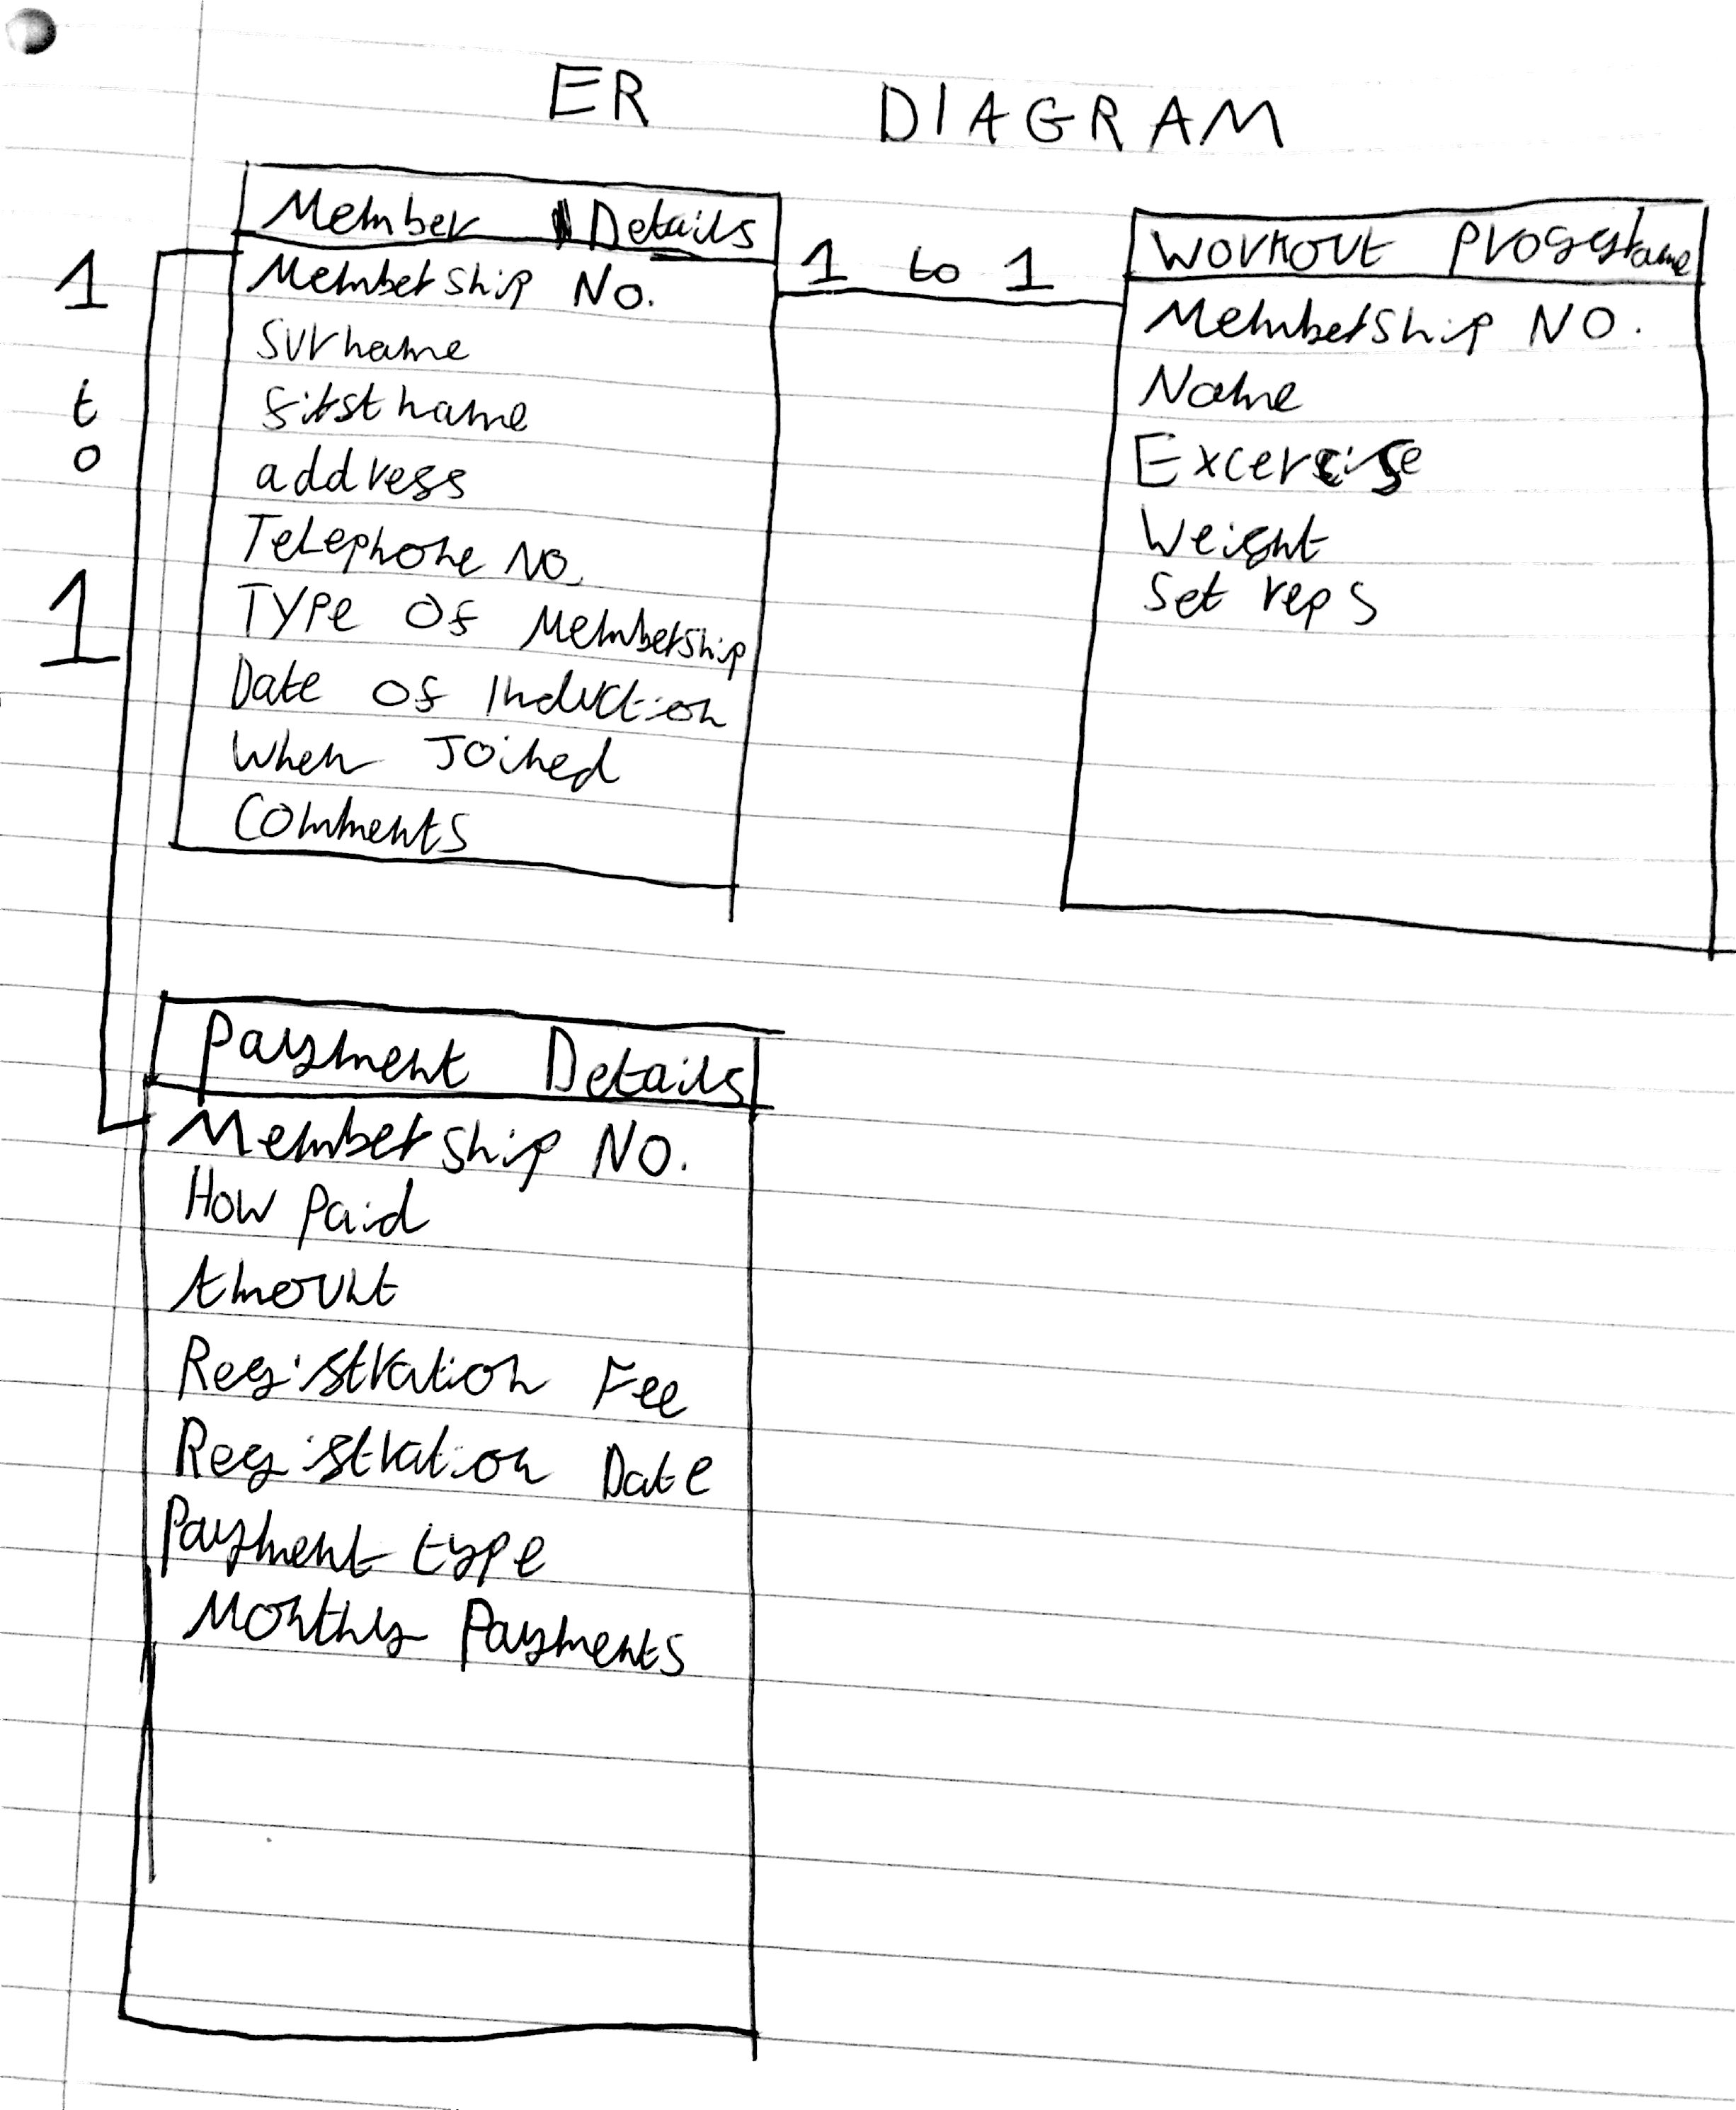
\includegraphics[width=\textwidth]{ER Diagram.jpg}
    \caption{ER Diagram} \label{fig: ER Diagram}
\end{figure}


\subsection{Entity Descriptions}

Membership Details(\textbf{\underline{Membership No.}}, Last Name, First Name, Address, Telephone No., Type Of Membership, Date of Induction, When Joined, Comments)

Payment Deatils(\textbf{\underline{Membership No.}}, How Paid, Amount, Registration Fee, Registration Date, Payment Type, Monthly Pay)

Workout Programme(\textbf{\underline{Membership No.}}, Excercise, Weight, Set Reps)

\section{Object Analysis}

\subsection{Object Listing}

\subsection{Relationship diagrams}

\subsection{Class definitions}

\section{Other Abstractions and Graphs}

Insert Gui Mock Ups Here

\section{Constraints}

\subsection{Hardware}

The owner currently uses a Notebook laptop powered by an intel 1st generation i5 processor and 4GB of RAM. He already uses this laptop to run his current system which uses more resources and power than this system will hopefully require, but if not he still has more than enough horse power to run the new system. His use of a laptop is convienient as it means his system is portable so he doesn't need to do any data entry (if required) confined to his office and away from his client if he doesn't want too and it also means he has a battery so in the case of a power outtage he wont lose any data. Though it is worth noting that he may soon be upgrading to a more powerful desktop soon so while this lowers portability, he has more power for the proposed system and he can easily have a battery backup in the form of a UPS(Uninterptable Power Supply).

The only hardware constraint this laptop proposes is the size and resolution of the screen. As it is only 1440p x 900p and 15 inches diagonally this doesn't give him much room to observe over 1300 clients without excessive amounts of scrolling. Fortunately this could be easily solved by either upgrading to a desktop or simply using an external monitor of a higher resolution.

\subsection{Software}

My client has no preference on what software can or cannot be used as long as its easily accessable to him as he isn't the most computer literate person. Its worth noting that although he has no particular requirements for software he isn't willing to learn a new operating system so it will have to run on windows 7. This is not a problem since the proposed system will be developed on a windows os and should be fully compatable.

\subsection{Time}

My client has given me no personal deadline for this project so the only one I have is the one set by AQA which at the time of writing is April 2015. Although my client doesn't need the new system immediately he is willing to use it as soon as possible and willing to test it before its finished providing its in a fully functioning state.

\subsection{User Knowledge}

Although the owner and staff members aren't specifically trained in I.T they are all completely able to use a computer when given the necessary instruction and support. Most of the staff only use computers for email and web browsing, and occasioinally writing things with a word processing package, as well as the current system which is computer based.

\subsection{Access restrictions}

Access to the proposed system should only be available to members of sweat gymnasium staff and thus the system may need a password although my client insists that only authorised people will have access to the computer, which is password protected itself so the password may be set to optional incase he wants to deactiate it. Due to the system containing private and confidential data on individuals it will have to comply with the Data Protection Act and appropriate action will be taken to do so though the care of the programs security is mostly in the hands of the staff and owner..

\section{Limitations}

\subsection{Areas which will not be included in computerisation}

\subsection{Areas considered for future computerisation}

\section{Solutions}

\subsection{Alternative solutions}

\subsection{Justification of chosen solution}